\documentclass[11pt, letterpaper,nounbold]{article}
\usepackage{mystyle}
\usepackage{indentfirst}
\pagestyle{plain}
\geometry{margin={0.6in}}

\usepackage{multicol}
\usepackage{optidef}

%%%%%%%%%%%%%%%%%%%%%%%
\renewcommand{\S}{\mathcal{S}}
\newcommand{\T}{\mathcal{T}}




\begin{document}

\section{Problem Proposal}
Modelling Canadian Heavy Crude Congestion pricing using Capacitated Transport networks 
Problem Proposal:

Alberta produces $\sim$4MM bbls/d (barrels per day) of crude oil of which $\sim$3 MM bbls/d is considered ``heavy oil''. Majority or 2/3 of Canadian heavy oil is consumed in PADD II and 1/3 in USGC refining center. The PADD III (also known as USGC - United States Coast Guard, see Figure~\ref{PADDsMap})  is considered a marginal consumption point for Canadian crude where the “last barrel” or marginal barrel is consumed. Canadian crude can reach the USGC through number of pipe options: Enbridge mainline, Express, and Keystone, or rail from either Edmonton or Hardisty. The cost of transport of the last barrel from Alberta to USGC is going to set the price of Canadian heavy benchmark (WCS) in Alberta. 

\begin{figure}[h!]
\centering
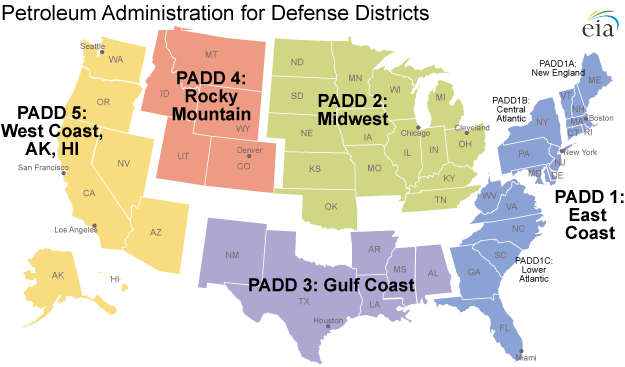
\includegraphics[scale=0.6]{PADDsMap}
\caption{Strategic and Military Pipeline for Transmission of Petroleum map. Available at \href{https://www.eia.gov/todayinenergy/detail.php?id=4890}{\nolinkurl{eia.gov}}} \label{PADDsMap}
\end{figure}


Pipe is considered a cheapest mode of transport of Canadian crude to the demand markets. The total offtake capacity from Alberta is on average less than the total available production. This leads often to the requirement of “call on rail” (the amount of rail capacity needed to clear an oversupply of barrels in the WCSB, see \href{https://atbcapitalmarkets.com/insights/north-american-crude-by-rail}{\nolinkurl{atbcapitalmarkets}}) or shut-ins (implementing a production cap lower than the available output of a specific site) to balance the market which in turn leads to significant price response. 
Prices are generally integrated if they respond to the same price shock. In reality looking at the USGC--Alberta spread pricing, we see a regular breakdown of the price relationship or ``congestion pricing'' (regulating demand by increasing prices without increasing supply). This is due to the fact that transient ``sub-markets'' can be form in a capacitated transport system.   


The question is using stochastic transport optimization (following a similar method to \cite{Pavlin2019} and \cite{Zhu2018}) can we model and answer the following questions:

\begin{itemize}
	\item When there are documented disruptions in the transport system can we predict how large the congestion surcharge was and how did prices respond to the disruption?
	\item Can we predict the occurrence of congestion by perturbing input factors in the system?
	\item How does shape and connections in the transport network contribute to the propensity for frequency of the congestion and magnitude of congestion surcharge?
\end{itemize}


There is a fantastic work performed looking at the US gasoline market that can be used as a guide ({\color{red} where is the guide?}) and starting point to look at the Canadian crude oil transport network.
The majority of the data: (1) Pipe Tolls and Tariffs (2) Capacities (3) Supply and Demand factors are publicly available. (4) Pricing data and some of the historical flow data that is used for benchmarking and testing the models can be made available with some degree of modifications and can be anonymized.      


\section{I. Y. Zhu's paper notes}
The competitive market is modeling with what we call the welfare-maximizing market allocation problem:
\begin{maxi*}|s|
{\vec{f},\vec{b}}{\sum_{s\in \mathcal{S}}W_{s}(b_{s}) - \sum_{(i,j)\in \mathcal{E}} c_{ij}f_{ij} - \sum_{k\in \mathcal{K}} W_{k}(b_{k}) }
{}{}
\addConstraint{-b_{s} + \sum_{i\in I(s)} f_{si} - \sum_{j\in O(s)} f_{sj} = 0, \qquad &\forall s\in \mathcal{S}}
\addConstraint{b_{k} + \sum_{i\in I(k)} f_{ik} - \sum_{j\in O(k)} f_{kj} = 0, \qquad &\forall k \in \mathcal{K}}{}
\addConstraint{0 \leq f_{ij} \leq u_{ij}, \quad \forall(i,j)\in \mathcal{E}}
\addConstraint{b_{s} \geq 0, \quad \forall s\in \mathcal{S}}
\addConstraint{b_{k} \geq 0, \quad \forall k\in \mathcal{K}}
\end{maxi*}
    \begin{multicols}{2}
    \begin{itemize}
        \item $\mathcal{S}, \mathcal{K}$ denotes the nodes in a network $\mathcal{N}$ populated by consumers and producers, respectively. 
        \item For a node $s\in \mathcal{S}$ ($k\in \mathcal{K}$), $W_{s}(b_{s})$ ($W_{k}(b_{k})$) is the welfare (production cost) for consuming (producing) $b_{s}$ ($b_{k}$) units. 
        \item Assume $W_{s}$ is strictly concave, increasing, and differentiable. Assume $W_{k}$ is convex, increasing and differentiable. 
        \item $\mathcal{E}$ denotes the set of transportation links $(i,j)$ from a node $(i,j)$ (i.e., it is the edge set of a directed graph)
        \item $f_{ij}$ denotes the flow from $i$ to $j$ on link $(i,j) \in \mathcal{E}$. $f_{i,j}$ is nonnegative, and bounded above by the capacity $u_{ij}$, with per-unit transportation cost $c_{i,j}$
        \item $I(j) = {(n,j) \in \mathcal{E}| n\in \mathcal{N}}$ The set of links that flow into the $j$th node from $n$.
        \item $O(i) = {(i,n) \in \mathcal{E} | n \in \mathcal{N}}$ The set of sets that flow out of the $i$th node to $n$.
        \item $\mathcal{P}(i,j)$ denotes the set of paths from $i$ to $j$, and $p_{ij}^{q}$ the cost of a path $q$ which is the sum of costs of the links from $i$ to $j$.
    \end{itemize}
    \end{multicols}
 In words, we are maximizing the welfare of the consumers less the cost of transportation and less the cost of production subject to the flow balancing, i.e., all that is produced is consumed.
 
\begin{defn}[Slater's condition]
For an optimization problem of the form 
	\begin{mini*}|s|
		{}{f_{0}(x)}{}{}
		\addConstraint{f_{i}(x) \leq 0, \qquad i = 1,\dots, m,}
		\addConstraint {Ax = b}
	\end{mini*}
If there exists an $x\in \operatorname{relint}\mathcal{D} = \cap_{i=0}^{m} \operatorname{dom}(f_{i})$ such that
	\[f_{i}(x) < 0, \qquad i = 1,\dots, m, \qquad Ax = b,\]
we say that the optimization problem satisfies \emph{Slater's condition}. That is, the optimization problem has an interior point in the feasible region. 
\end{defn}
\begin{theorem}
Given the following optimization problem 
	\begin{align*}
		&\text{Optimize}\qquad  f(\mathbf{x})\\
		&\text{Subject to}\\
		&\qquad g_{i}(\mathbf{x})\leq 0,\,  h_{j}(\mathbf{x}) = 0.
	\end{align*}
with associated Lagrangian
	\[L(\mathbf{x}, \mu,\lambda) = f(\mathbf{x}) + \mu^{T}\mathbf{g(x)} + \lambda^{T}\mathbf{h(x)}.\]
Let $x^{\star}$ and $(\lambda^{\star}, \mu^{\star})$ be any primal and dual optimal points with zero duality gap. Then $x^{\star}$ is the minimizer of $L(x, \lambda^{\star}, \mu^{\star})$ and hence its gradient vanishes at $x^{\star}$,
	\[\nabla f_{0}(x^{\star}) + \sum_{i=1}^{m} \lambda_{i}^{\star} \nabla f_{i}(x^{\star}) + \sum_{i=1}^{p}\mu_{i}\nabla h_{i}(x^{\star}) = 0.\]	
In particular,
	\begin{align*}
		f_{i}(x^{\star}) &\leq 0,\qquad  i = 1, \dots, m\\
		h_{i}(x^{\star}) &= 0,\qquad  i = 1\dots, p\\
		\lambda_{i}^{\star} &\geq 0,\qquad  i = 1,\dots, m\\
		\lambda_{i}^{\star}f_{i}(x^{\star}) &= 0,\qquad  i = 1,\dots, m.
	\end{align*}
These four equations together with 
	\[\nabla f_{0}(x^{\star}) + \sum_{i=1}^{m} \lambda_{i}^{\star} \nabla f_{i}(x^{\star}) + \sum_{i=1}^{p}\mu_{i}\nabla h_{i}(x^{\star}) = 0\]
are known as the \emph{Karush--Kuhn--Tucker} (KKT) conditions. For any convex optimization problem with differentiable objective and constraint functions, any points that satisfy the KKT conditions are primal and have zero duality gap. Further, if Slater's condition is satisfied, these conditions are necessary and sufficient for optimality. See \cite[Ch.~5]{Boyd2009}
%If $(\mathbf{x}^{*}, \mu^{*})$ is a saddle point of $L(\mathbf{x}, \mu)$, $\mathbf{x}$ in a convex set $\textbf{X}$ and $\mu \geq 0$, then $\mathbf{x}^{*}$ is an optimal vector for the above optimization problem. Furthermore, of $f$ and $g_{i}$ are convex in $\mathbf{x}$ and there exists $\mathbf{x_{0}}\in \mathbf{X}$ such that $\mathbf{g}(\mathbf{x}_{0}) < 0$. Then associated with $\mathbf{x}^{*}$ there exists a nonnegative $\mu^{*}$ such that $L(\mathbf{x}^{*}, \mu^{*})$ is a saddle point. 
\end{theorem}

\section{Discussion with Nima}
\subsection{Data sources}
There are several sources of data that we can use for this project:
\begin{itemize}
	\item The US Energy Information Administration, \url{https://www.eia.gov/maps/}, contains maps that can be filtered to show the crude pipelines and an interactive map displaying all the refineries and other data.
	\item The Alberta Energy Regulator, \href{https://www.aer.ca/providing-information/data-and-reports/statistical-reports/st98/statistics-and-data.html}{here} provides an annual energy report and includes the data sets used to generate the reports known as the ST98. Also see the statistical reports available \href{https://www.aer.ca/providing-information/data-and-reports/statistical-reports.html}{here}.
	\item Oil Sands Magazine \url{https://www.oilsandsmagazine.com/projects/crude-oil-liquids-pipelines} has a lot of data including maps that show the toll rates for oil and the production capacity at various sites.
\end{itemize}
\subsection{Market characteristics}
There are many miscellaneous market characteristics of note that are written here:
\begin{itemize}
	\item{Rail is the most expensive method of transport and costs \$17 per barrel. The total rail capacity is 300,000 barrels per day.}
	\item{WCS trades as a basis to WTI. That is, if WCS is \$40 and WTI \$50, it is often said that WCS is -\$10. That is, WCS is worth \$10 less than WTI. This basis is taken to include the difference in transportation costs from Alberta to Cushing, and a grade adjustment. The grade adjustment is said to be negligible. Further, note that the differential between Heavy and Light oil is about \$5 per barrel.}
	\item{Note that as a result of COVID-19, the demand for US oil dropped from 17mm barrels to 13mm barrels per day. Given that Canada only produces 4mm barrels per day, this was a substantial drop in demand.}
	\item{There are two notable sources of pipeline disruption. The most notable source of disruption are related to the keystone pipeline. In particular, Nima recalls a disruption in 2019 in possibly November or December, and a disruption in 2017 in January.}
	\item{Traders use what is known as a calendar month average. I don't think this will be too important but remember this when considering how traders might work.}
	\item{The oil price spreads generally follow a mean reverting process, so an OU process is going to be a good candidate.}
\end{itemize}

\section{SEM with constraints}
\begin{align*}
z(\beta) : = \text{minimize \qquad } &\sum_{s\in \S} \alpha_{s}\\
	\text{subject to \qquad} &\lambda_{s}^{t} = \eta^{t} + \rho_{s} + \epsilon_{s}^{t} + w_{s}^{t},\qquad \forall s \in \S, t \in \T,\\
		& \epsilon_{s}^{t} \geq -\alpha_{s},\qquad \forall s\in \S, t \in \T\\
		& \epsilon_{s}^{t} \leq \alpha_{s},\qquad \forall s\in \S, t\in \T\\
		& w_{s}^{t} \leq \psi^{t}M, \qquad \forall s\in \S, t \in \T,\\
		&\sum_{t\in \T} \psi^{t} \leq \lfloor \beta T\rfloor\\
		&w_{s}^{t} \leq \pi_{s}^{t} M, \quad \forall s\in \S, t \in \T\\
		&\epsilon_{s}^{t} + (1-\pi_{s}^{t})M \geq \alpha_{s}, \qquad \forall s\in \S, t\in \T,\\
		&\sum_{s}\gamma_{s}^{t} \geq \psi^{t}, \forall t\in \T\\
		&\epsilon_{s}^{t} \leq -\alpha_{s} + (1-\gamma_{s}^{t})M, \qquad \forall s\in \S, t\in \T\\
		&\gamma_{s}^{t}, \psi^{t}, \pi_{s}^{t}\in \{0, 1\}, \qquad \forall s\in \S,t\in \T\\
		&w_{s}^{t} \geq 0 \qquad \forall s\in \S, t\in \T
\end{align*}
Note that under the change of variables $\overline{w}_{s}^{t}: = w_{s}^{t} + \epsilon_{s}^{t} - \alpha_{s}$, this can be simplified to
\begin{align*}
z(\beta) : = \text{minimize \qquad } &\sum_{s\in \S} \alpha_{s}\\
	\text{subject to \qquad} &\lambda_{s}^{t} = \eta^{t} + \rho_{s} + \alpha_{s} + \overline{w}_{s}^{t},\qquad \forall s \in \S, t \in \T,\\
		& \overline{w}_{s}^{t} \geq -2\alpha_{s},\qquad \forall s\in \S, t \in \T,\\
		& \overline{w}_{s}^{t} \leq \psi^{t} M,\qquad \forall s\in \S, t\in \T,\\
		&\sum_{t\in \T} \psi^{t} \leq \lfloor \beta T\rfloor,\\
		&\overline{w}_{s}^{t} \leq -2\alpha_{s} + (1-\gamma_{s}^{t})M, \qquad \forall s \in \S, t\in \T,\\
		&\sum_{s}\gamma_{s}^{t} \geq \psi^{t},\qquad \forall t\in \T,\\
		&\gamma_{s}^{t}, \psi^{t} \in \{0,1\}, \qquad \forall t\in \T.
\end{align*}
Given optimal values of $\overline{w}_{s}^{t}$ we can return to the original $w_{s}^{t}$ and $\epsilon_{s}^{t}$ as follows: If $\overline{w}_{s}^{t} \geq 0$, then $w_{s}^{t} = \overline{w}_{s}^{t}$ and $\epsilon_{s}^{t} = \alpha_{s}$. If $\overline{w}_{s}^{t} < 0$, then $w_{s}^{t} = 0$ and $\epsilon_{s}^{t} = \overline{w}_{s}^{t} + \alpha_{s}$. Note that for larger data sets, we may need to use an additional set of constraints to reduce the scope of the problem. See \cite[pp.~23--24]{Zhu2020} for details.
\subsection{SEM notes}
This model takes as an input a set of spatial prices $\pmb{\lambda} = \{\lambda_{s}^{t}\}_{s\in \S, t\in \T}$ and returns an estimate of congestion over a given time horizon. The variable $\eta^{t}$ captures a node-invariant underlying trend, $\rho_{s}, \epsilon_{s}^{t}$, and $\alpha_{s}$ capture time-invariant neutral bands. All the remaining price variation is captured by the variables $w_{s}^{t}$ representing surcharges. We represent the constraints on $w_{s}^{t} by \mathcal{W}\subseteq \mathbb{R}^{+}$. That is, $\mathcal{W}$ restricts the domain of $w_{s}^{t}$.

If prices differences are perfectly constant , theoptimal objective value will be zero and the prices $\lambda_{s}^{t}$ can be explained entirely by the node-invariant $\eta^{t}$ and the time-invariant $\rho_{s}$. Consider perturbing the $\lambda_{s}^{t}$ with Ornstein--Uhlenbeck stochastic processes to avoid this. Similarly, we can use this as a test that the optimization routine is working.

The parameters
	\[w_{s}^{t} \leq \psi^{t} M, \sum_{t\in \T} \psi^{t} \leq \lfloor \beta T\rfloor, \psi^{t} \in \{0,1\}\]
represent time constraints. The parameter $\psi^{t}$ is an indicator variable for when the congestion surcharge is free ($\psi^{t} =1$) or fixed to zero ($\psi^{t} = 0$). The parameter $M$ represents a large value such that $w_{s}^{t}$ will never reach its upper bound when $\psi^{t} = 1$. Finally $\beta$ is a fraction of time periods for which the underlying network is congested. The remaining $\lceil (1-\beta) T\rceil$ periods with no congestion (and hence $\psi^{t} = 0$) are used to fit $\rho_{s}$  so that we can precisely estimate $w_{s}^{t}$ when $\psi^{t} = 1$. The goal of these is to ensure that $\eta^{t}$, (resp.~$w_{s}^{t}$) are the largest (resp. smallest) possible value out of the set of optimal solutions.
\subsubsection*{Questions}
What is $\alpha_{s}$? It must be $\lambda_{s}-W^{\prime}_{s}(b_{s})$ from \cite[p.~7]{Zhu2020}
\bibliographystyle{amsplain}
\bibliography{project}

\end{document}
